
\documentclass[12pt]{iopart}
\usepackage{iopams}  
\usepackage{braket}
\usepackage{graphicx}
\usepackage{subfigure}
\usepackage{cite}
\usepackage{algorithm}
\usepackage{algorithmic}



\begin{document}
\newcommand{\swave}[0]{$\it{s}$-wave }
\newcommand{\pwave}[0]{$\it{p}$-wave }
\newcommand{\K}{ $^{40}\rm{K}$}
\newcommand{\Rb}{ $^{87}\rm{Rb}$}
\newcommand{\us}{$\mu \rm{s}$} 

\title[]{Direct observation of Feshbach enhanced \swave scattering of fermions}

\author{D Genkina$^1$, LM Aycock$^{1,2}$, BK Stuhl$^1$, H-I Lu$^1$ and IB Spielman
$^1$\footnote{Corresponding author}}

\address{$^1$Joint Quantum Institute, National Institute of Standards and Technology, and University of Maryland, Gaithersburg, MD, 20899 USA}
\address{$^2$Physics Department, Cornell University, Ithaca, NY 14850 USA}

\ead{ian.spielman@nist.gov}

\begin{abstract}
We directly measured the \swave{} scattering cross-section of \K atoms accross a Feshbach resonance. We collided a pair of degenerate clouds and imaged the scattered atoms. Owing to their low density, few atoms scattered, even near the resonance. To optimize signal to noise, we develop techniques to interpret absorption imaging in the regime where the optical intensity changes dramatically as light traverses the cloud, and recoil induced 
detuning corrections are significant. We applied these techniques to our \swave{} scattering data and extracted the resonant magnetic
field value. These imaging techniques are generally applicable, and can be used to observe effective \pwave{} scattering in the presence of spin-orbit coupling in a spin polarized  Fermi gas.

\end{abstract}

\vspace{2pc}
\noindent{\it Keywords}: Quantum gases, Atomic physics

\maketitle

\section{Introduction}
Feshbach resonances are a stand-by technique for tuning the interaction strength in ultracold atomic gases. Even weak interactions play a crucial role in the physics of atomic Bose-Einstein Condensates (BECs), giving rise to, for example, their characteristic Thomas-Fermi density profiles. The effects of interactions in Fermi gases, however, are harder to observe. The density of Fermi clouds is typically reduced by a factor of $~10^3$ from that of BECs, making it necessary to enhance the strength of interactions in order to observe them. Feshbach resonances alter the inter-atomic scattering length via the magnetic field. Not only do they enable detection of interactions, but they make it possible to tune interactions from attractive to repulsive, allowing for the phase transition from the BCS to BEC regime at sufficiently low temperatures \cite{RegalThesis}. 
\par A Feshbach resonance occurs when a bound molecular state of few atoms energetically approaches the free atomic state \cite{Chin10}. The energy of the atomic states is defined by their hyperfine state and tunable with a bias magnetic field. The Feshbach resonance can thus be approached by changing the bias field. The effect of the resonance on the scattering length between two free atoms in the appropriate hyperfine states is
\begin{equation}
a(B)=a_{bg}\left(1-\frac{\Delta}{B-B_0}\right),
\label{feshbachEq}
\end{equation}
where $a$ is the scattering length, $a_{bg}$ is the scattering length away from the resonance, $\Delta$ is the width of the resonance, and $B_0$ is the field value at which the resonance occurs. Note that the scattering length tends to infinity from either side of the resonance.
\par To use Feshbach resonances as a tool it  is necessary to have a good measurement of the parameters in the above equation.  The exact value of the resonant field value $B_0$ is impossible to calculate analytically and must be estimated via numerical models \cite{Lysebo09, Gao11} or determined experimentally. Some experimental techniques that have been used to characterize Feshbach resonances include: the observation of loss due to three-body inelastic scattering, re-thermalization timescales, or anisotropic expansion, all of which infer the elastic scattering cross section from collective behavior of the cloud \cite{Regal03,OHara02,Monroe93}. 
\par Here we present a new technique for measuring the location and width of a Feshbach resonance. We collide a pair of ultra-cold Fermi gases and directly image the resulting \swave scattering halo as a function magnetic field strength. This allows us to observe the enhancement in scattering without relying on proxy effects. We measured the fraction of atoms scattered during the collision, and from this fraction deduced the resonant magnetic field  and width of the resonance.
%\par The techniques developed in this experiment for observing Fermion scattering can be extended to engineering higher order partial wave interactions, as has been done for bosons \cite{Williams2012}.
\par Our Fermi gases are so dilute that even with the resonant enhancement of the scattering cross section, only a small fraction of the atoms scatter. This makes direct detection of \swave scattering halos difficult due to detection uncertainty, which disproportionately affects regions of low atomic density. To optimize the signal to noise for low atom numbers, we utilized a non standard imaging regime. In this regime, simulation was necessary for an accurate interpretation of the images. We performed these simulations and used the results to extract the atom number and the scattered fraction from our images.
\par This paper is in two parts. In the first, we study absorption imaging in the presence of significant time-dependent Doppler shift and show how we use our results to interpret data. In the second, we describe our\swave scattering experiment and extract a measure of the location of the Feshbach resonance in \K. 

\section{Absorption imaging in the presence of strong recoil induced detuning}
Every experiment requires a detection scheme. In ultracold atomic experiments, detection relies on imaging laser light that has interacted in some way with the atomic cloud. The most common such imaging method, and the one we use in our experiments, is absorption imaging. Absorption imaging utilizes some excited to ground state transition between two levels of the atom. Such an atomic transition has an energy difference $E_0$, an associated frequency $\omega_0 = E_0/\hbar$, and a natural transition linewidth $\Gamma$. When interacting with a laser light field an atom will scatter photons: if will absorb a photon from the light field and move up to its excited state, and then re-emit the photon in a random direction and decay back to its ground state. The  rate at which this scattering occurs, given a laser intensity $I$, is given by
\begin{equation}
\gamma_{sc}= \frac{\Gamma}{2} \frac{I/I_{sat}}{1+(2\delta/\Gamma)^2 +I/I_{sat}}, 
\label{eq:scatrate}
\end{equation}
where $I_{sat}$ is the saturation intensity, the intensity at which the atom is equally likely to be in the ground and excited state, and $\delta$ is the detuning, the difference between the resonant transition frequency $\omega_0$ and the frequency of the laser light $\omega_L$.  
\par To obtain an absorption image, one shines an on or near resonant probe beam ($\delta\approx0$) onto the atomic cloud. Some of the light is scattered by the atoms, and the part of the beam that made it through the cloud is imaged onto a camera, as seen in Fig. \ref{fig:absorptionIntor}a (top). Then, the atoms are allowed to leave the trap, and the probe light is shined directly at the camera to calibrate the intensity of light that the atoms saw (bottom). The intensity in the second camera image is called the initial intensity, $I_{0}$, as it is assumed to be the same as the intensity in the first beam before interaction with atoms. The intensity in the first image is called the final intensity, $I_f$.  
\begin{figure}
	\subfigure[]{\includegraphics*[scale=0.55]{Picture1a}}
	\subfigure[]{\includegraphics*{Picture1c.pdf}}
	\subfigure[]{\includegraphics*[scale=0.55]{Picture1b}}
\caption{Absorption imaging. a. First, a near resonant probe light is shined on the atoms, and the shadow of that light is imaged on the camera. Then, the atoms are allowed to escape their trap and an image of just the probe light is taken. b.  As the probe beam, travels through the atomic cloud, some of its power is absorbed, and the intensity seen by atoms further along the imaging direction $z$ is lowered.  c. An atomic cloud illuminated by a probe light field absorbs photons from the probe and re-emits them in arbitrary directions. This process results in a net velocity of the cloud in the direction of the probe light as well as diffusive spreading in the transverse directions.  }  
\label{fig:absorptionIntor}
\end{figure}
\par The observed intensity in the two images can be used to infer the number of atoms that the light encountered. To do this, consider what happens to the light as it travels along the imaging axis $z$ through a column of atoms. In general, the atomic density is three dimensional, $\rho(x,y,z)$. For the purposes of this discussion, let us focus on a single pixel of the camera, and thus a single value of $I_0$ and $I_f$ and a single column of atoms, $\rho(z)$. We will not be able to infer the entire atomic distribution, but for each pixel we will be able to deduce the total 2-d atomic density, $n = \int \rho\left(z\right) \,\mathrm{d}z$. As the light travels through a column of atoms, each atom will scatter light according to Eq. (\ref{eq:scatrate}). Therefore, the atoms further along the imaging axis $z$ will see a reduced light intensity, as seen in Fig. \ref{fig:absorptionIntor}b. The amount of light lost to scattering as a function of $z$ is given by
\begin{equation}
\frac{dI(z)}{dz}=\hbar\omega_L\rho\gamma_{sc}=-\rho\sigma_0\frac{I(z)}{1+I(z)/I_{sat}},
\end{equation}
where $\sigma_0$ is the resonant scattering cross section. We have assumed $\delta=0$. 
 This equation can be easily integrated over $z$ to obtain  \cite{Reinaudi07}
\begin{equation} 
\sigma_0 n = -\ln\left(\frac{I_f}{I_0}\right) + \frac{I_0-I_f}{I_{sat}}.
\label{eq2}
\end{equation}
In the limit where the probe intensity is much smaller than the saturation intensity, $I_0\ll I_{sat}$, this becomes simply $-\ln \left(I_f/I_0\right)$. This quantity is called the optical depth, or OD. Since this is the simplest possible model that relates the observed intensities to the column density $n$, we call this quantity $OD_0$. Once the probe intensity becomes comparable to the saturation intensity, the second term in Eq. (\ref{eq2}) becomes significant. We can then call this the optical density corrected for high probe intensity, or
\begin{equation} 
OD_1 = OD_0 + \frac{I_0-I_f}{I_{sat}}.
\label{eq:OD1}
\end{equation}
There are further corrections that this equation does not take into account. In particular, it neglects the atomic recoil momentum and its effect on the laser detuning, which will be discussed below.
\par When an atom absorbs a photon from the laser light field and gets excited to a higher energy level, by conservation of momentum it must also acquire a velocity in the direction of the light field. This is called the recoil velocity, and it is given by $v_r=\hbar k/m$, where $k$ is the wavenumber of the light field and $m$ is the atomic mass. When the photon is subsequently emitted and the atom returns to its ground state, it is emitted in an arbitrary direction. Thus, the momentum lost due to emitting a photon is on average zero. The variance, however, is not zero, allowing the atoms to acquire some momentum transverse to the laser field. We will ignore this correction, but the effect of this on the atomic cloud is picture in Fig. \ref{fig:absorptionIntor}c. 
\par Once the atoms absorb enough photons, they acquire a substantial velocity in the direction of the light field, and this velocity Doppler shift them from the light field itself. Thus, an atom that absorbs $N$ photons acquires a velocity of $N v_r$ and a detuning of $\delta=k N v_r$ from the probe beam. Therefore, even if the probe beam is initially on resonance with the atomic transition, we cannot neglect the detuning term in the scattering rate as time goes on. Furthermore, this detuning will vary both with imaging time $t$ and with distance along the propagation direction $z$ (Fig. \ref{fig:detunedBlobs}). Thus, the intensity lost to the atoms also acquires a time dependence: 
\begin{equation}
\frac{dI(t,z)}{dz}=\sigma_0 \rho \frac{I(t,z)}{1+(2\Gamma/\delta(t,z))^2 +I(t,z)/I_{sat}}, \label{eq3}
\end{equation}
where the detuning $\delta$ is given by 
\begin{equation}
\delta(t,z)=\frac{v_r}{\hbar c \rho}\int_0^t \frac{dI(z,\tau)}{dz}\,\mathrm{d}\tau. \label{eq4} 
\end{equation}
In this case, one can no longer obtain a straightforward relation between the atom number and the intensities in the two absorption images.
\begin{figure}
	\includegraphics*{figure1.pdf}
\caption{Distribution of generalized detuning $\Delta=\frac{2\delta}{\Gamma}$ across an atomic cloud of $^{40}K$ for three different imaging times, as obtained by numerical simulation.}  
\label{fig:detunedBlobs}
\end{figure}
\par One can consider this equation perturbatively in time and obtain corrections to second order in imaging time, $OD_2$  \cite{LJLthesis}. However, the perturbative treatment breaks down shortly after the zeroth order approximation of Eq. (\ref{eq2}) (Fig. \ref{fig:ODcorrections}). In order to adequately correct for the recoil induced detuning of the atoms, we must simulate the process and obtain numerical predictions for $I_f$ given a certain imaging time, atomic density, and probe intensity. 
\begin{figure}
	\includegraphics*{figure2.pdf}
\caption{Using time dependent $I_f$ values obtained from recoil detuning corrected simulation of on-resonant imaging of $^{40}K$ atoms, this graph shows the optical depths each model would deduce from such images. The true optical depth is given at 1.6.$OD_1$ is the high probe intensity corrected optical depth given by \ref{eq2}. $OD_2$ is the model that includes high probe intensity corrections and imaging time corrections from expanding \ref{eq3},\ref{eq4} to second order in imaging time \cite{LJLthesis}. Note that the value obtained using the second order expansion in time starts to differ significantly from the true value after about 15us. The probe intensity is $0.8\, I_{sat}$. }  
\label{fig:ODcorrections}
\end{figure}
\par In the following, we describe two versions of this simulation. First, we take the simplistic approach that the on-axis distibution of atoms does not change dramatically durning the imaging time and can be treated statically. We test this approach in known limits and then check the validity of the static assumption. It turns out that, for realistic input parameters, this assumption is grossly incorrect. So, we take a slightly more sophisticated approach and allow the atoms to move within the cloud during the imaging time. This allows us to simulate the phase space evolution of atoms subjected to probe light. However,   
 we find that  while the atomic trajectories are wildly different, the predicted ODs only vary on the 0.5$\%$ level between the two models. 


\subsection{Stationary atom model}
In order to solve eqs. [\ref{eq3}]-[\ref{eq4}], we start with an input 1-d distribution of atom densities $\rho(z)$, usually Gaussian in shape. We divide the cloud into spatial bins (the bin size was chosen such that decreasing the bin size further produced less than a 0.001$\%$ difference in the result).  In this approximation, we keep the number of atoms in each bin constant.  The algorithm used is shown in alg. [\ref{algorithm1}]. We call the optical depth obtained from this algorithm $OD_{corr1}$.

\begin{algorithm}
\caption{Stationary atom model}
\label{algorithm1}
\begin{algorithmic}
\STATE $I[n=0,t]=I_0$ \COMMENT{$n$ is the bin index, $t$ is the time index, $I$ is in units of $I_{sat}$} 
\STATE $\delta[n, t=0]=0$ \COMMENT{light initially resonant, $\delta$ in units of $\Gamma/2$}
\STATE $I_f=0$
\FOR[loop over time steps]{$t=0$ to $t_f$}
 \FOR[loop over bins, N is total bin number]{$n=1$ to $N$}
 \STATE $A=\sigma_0\rho[n] dz$
 \STATE $B=v_r dt/(\hbar c \rho[n])$ 
\STATE $I[n,t]=I[n-1,t] - A I[n-1,t]/(1+\delta[n,t-1]^2+I[n-1,t])$  \COMMENT{Eq. (\ref{eq3})}
\STATE $\delta[n,t]=\delta[n,t-1]+B\left(I[n-1,t]-I[n,t]\right)$  \COMMENT{Eq. (\ref{eq4})} 
\ENDFOR 
\STATE $I_f  \mathrel{+}= I[N,t]dt$
\ENDFOR
\STATE $OD_{corr1}=-\ln{(I_f/I_0t_f)}$
\end{algorithmic}
\end{algorithm}

\par To check the validity of our simulation, we can take it to certain limits in which the problem becomes analytically solvable. In the limit that the probe intensity is much weaker than saturation, $I_0\ll I_{sat}$, the atoms will not absorb enough light to significantly detune from resonance. We can then neglect time dependence and Eq.(\ref{eq3}) reduces to 
\begin{equation}
\frac{dI(z)}{dz}=-\rho\sigma_0 I(z),
\end{equation}
from which we recover the simple
\begin{equation}
\sigma_0 n = OD_0 = -\ln I_0/I_f. \label{eq6}
\end{equation}
In the limit that the probe intensity is much stronger than saturation, $I_0\gg I_sat$, even far detuned atoms will absorb light at their maximum, allowing us to again neglect the time dependence and reduce \ref{eq3} to 
\begin{equation}
\frac{dI(z)}{dz}=-\rho\sigma_0 I_{sat}, 
\end{equation}
which integrates to 
\begin{equation}
\sigma_0 n = \frac{I_0 - I_f}{I_{sat}}. \label{eq8}
\end{equation}
We recognize the right hand sides of Eq. (\ref{eq6}) and Eq. (\ref{eq8}) as the two terms in the expression for $OD_1$, Eq. (\ref{eq2}). Thus, in both limits $OD_{corr1}$ should coincide with the value of $OD_0$ obtained by fixing an input atom number $n$ in Eq. (\ref{eq2}). Indeed, they coincide as seen in Fig. \ref{fig:IsatLimits}.
\begin{figure}
	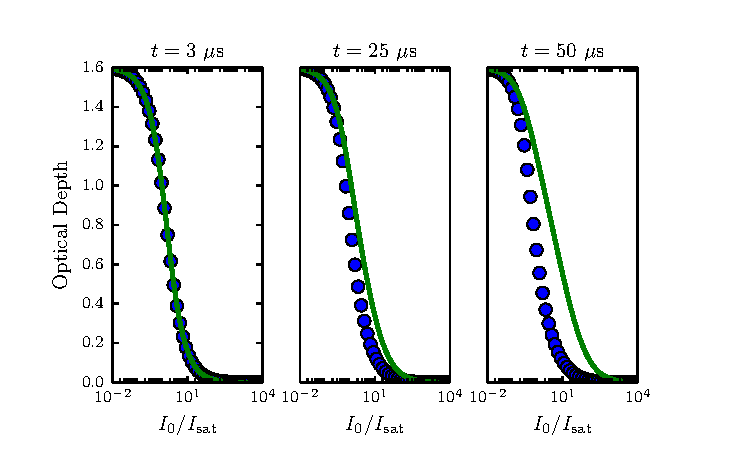
\includegraphics{figure3.pdf}
\caption{Optical density as a function of probe intensity as predicted by the simulation (blue dots) and by Eq. (\ref{eq6}) (green lines), for three different imaging times. The predictions agree in both the high and low intensity limits, and differ for probe intensities comparable to the saturation intensity. The difference is enhanced with increased imaging time.}  
\label{fig:IsatLimits}
\end{figure}
\par We can use the results of this simulation to check if the stationary atom assumption is self consistent, ie if the distance traveled by the atoms in one bin during the imaging time is less than the bin size. However, as can be seen from Fig. \ref{fig:atomTravel}, it turns out that not only do the atoms travel more than the bin size, but they also travel more than the size of the whole cloud, and the back of the cloud even overtakes the front for long enough imaging times. Thus, the atomic distribution as a function of position changes dramatically during the imaging time, and our stationary assumption is completely invalid. 
\begin{figure}
	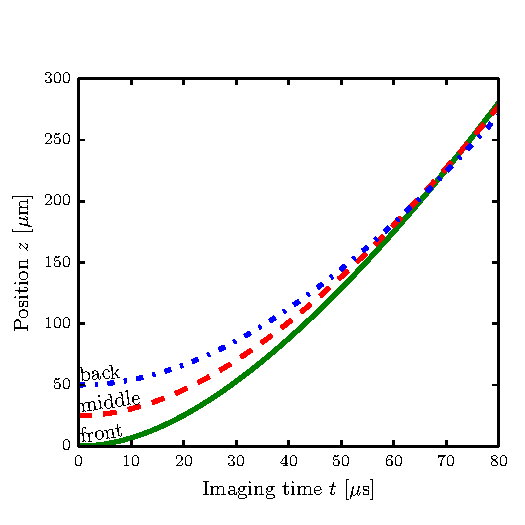
\includegraphics{figure4.pdf}
\caption{Position of atoms as a function of imaging time for atoms in the first, middle, and last bins of the simulation. The probe intensity here is $1.2 I_{sat}$, and the optical depth is 1.6.}  
\label{fig:atomTravel}
\end{figure}

\subsection{Traveling atom model}
To account for the changing atomic distribution during the imaging pulse, we shift our framework slightly from spatial bins of equal size with varying atoms number to superatoms. These superatoms were spatially distributed to match a typical experimental distribution, each describing the aggregate behavior of $N_{sa}$ atoms. The amended algorithm is shown in alg.[\ref{algorithm2}]. 
\begin{algorithm}
\caption{Travelling atom model}
\label{algorithm2}
\begin{algorithmic}
\STATE $S[n]=\mathrm{Superatom}(z=z_0[n], \delta=0)$ \COMMENT {initialize array of superatom class instances, with position and detuning attributes} 
\STATE $I[n=0,t]=I_0$ \COMMENT{ $t$ is the time index, $I$ is in units of $I_{sat}$} 
\STATE $I_f=0$
\FOR[loop over time steps]{$t=0$ to $t_f$}
 \FOR[loop over superatoms]{$n=1$ to $N$}
 \STATE $A=\sigma_0 N_{sa} dz$
 \STATE $B=v_r dt/(\hbar c  N_{sa})$ 
\STATE $I[n,t]=I[n-1,t] - A I[n-1,t]/(1+S[n].\delta^2+I[n-1,t])$  \COMMENT{Eq. (\ref{eq3})}
\STATE $S[n].\delta\mathrel{+}=B\left(I[n-1,t]-I[n,t]\right)$  \COMMENT{Eq. (\ref{eq4}), detuning in units of $\Gamma/2$} 
\STATE $S[n].z\mathrel{+}=dt\Gamma\delta/2k$ \COMMENT{$k$ is the wavenumber, $\Gamma\delta/2k$ is the velocity at $\delta$ detuning}
\ENDFOR 
\STATE $S[n]$=sort($S[n]$, key =$\mathrm{ Superatom}.z$) \COMMENT{sort superatoms by current position}
\STATE $I_f  \mathrel{+}= I[N,t]dt$
\ENDFOR
\STATE $OD_{corr2}=-\ln{(I_f/I_0t_f)}$
\end{algorithmic}
\end{algorithm}
\par First, we check the velocity behavior in this model against known limits. One such limit is that of a single supeatom. In this case, there is no attenuation, and the intensity seen by the superatom is constant at $I_0$. The only thing that evolves in time is the detuning of the single superatom. We can differentiate both sides of Eq. (\ref{eq4}) to obtain
\begin{equation}
\frac{d\delta\left(t\right)}{dt}=\frac{v_r}{\hbar c \rho}\frac{dI}{dz},
\label{eq9}
\end{equation} 
and Eq. (\ref{eq3}) simplifies to
\begin{equation}
\frac{dI}{dt}=\frac{v_r \sigma_0}{\hbar c}\frac{I_0}{1+(2\delta(t)/\Gamma)^2 +I_0/I_{sat}}.
\label{oneAtom}
\end{equation}
Combining Eq. (\ref{eq9}) and Eq. (\ref{oneAtom}), and converting to a dimensionless form, we obtain
\begin{equation}
\frac{d\Delta(t)}{dt}= k v_r \frac{\tilde{I}}{1+\Delta^2+\tilde{I}},
\label{eq10}
\end{equation}
where $\Delta = 2\delta/\Gamma$, $\tilde{I} = I_0/I_{sat}$ and $k$ is the photonic wavevector. Equation (\ref{eq10}) can be solved numerically, and is in good agreement with our simulation, as seen in Fig. \ref{fig:oneAtomVel}.
\begin{figure}
	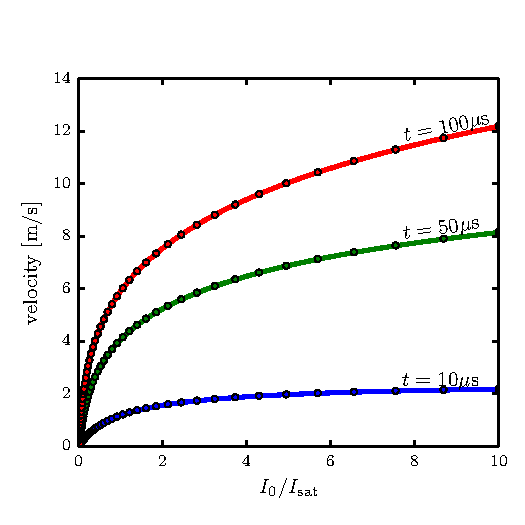
\includegraphics{figure5.pdf}
\caption{The velocity of a single superatom as a function of probe intensity for various imaging times. Simulation data (dots) and analytical solutions (lines) are in good agreement.}  
\label{fig:oneAtomVel}
\end{figure}
\par We use this model to study the time evolution of the cloud shape during imaging. This can be visualized as the phase space evolution of superatoms, as seen in Fig. \ref{fig:phaseSpace}. We see that the cloud shape is actually strongly distorted during the imaging time. 
\begin{figure}
	\subfigure[]{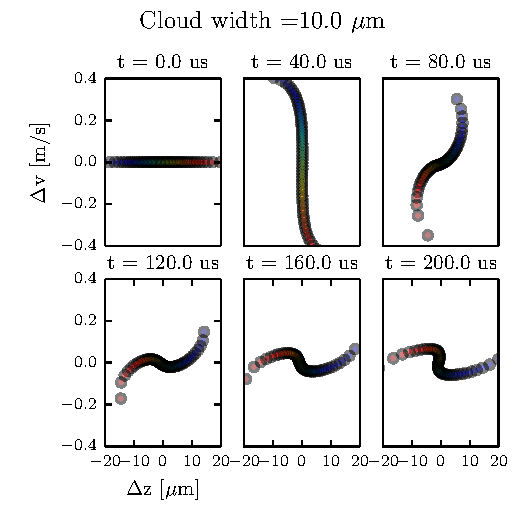
\includegraphics{figure6a.pdf}}
	\subfigure[]{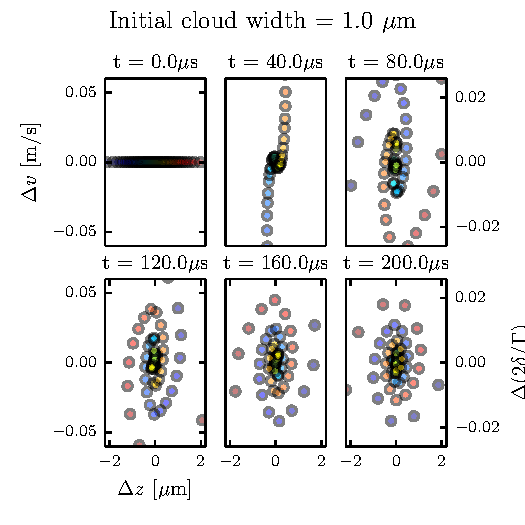
\includegraphics{figure6b.pdf}}
\caption{Phase space evolution of an atomic cloud exposed to probe light of $1.2 I_{sat}$. We have used $\Delta \rm{v}=\rm{v} -\left< \rm{v}(t) \right>$  and $\Delta \rm{z}=\rm{z}-\left< \rm{z}(t) \right>$, subtracting out the center of mass position and velocity of the cloud. The optical depth is 1.6, and the initial cloud is a gaussian with width a.10$\mu m$ and b.1$\mu m$.}  
\label{fig:phaseSpace}
\end{figure}
\par We compare the optical depths predicted by each of the two models, $OD_{corr1}$ and $OD_{corr2}$. We find that, depite the significant changes in atomic distribution during the imaging time, the predicted optical densities are so slightly changed by including this effect that it is practically undetectable, as seen in Fig. \ref{fig:atomTravel}. In fact, the difference $\left|OD_{corr1}-OD_{corr2}\right|/OD_{corr1} \le 0.005$. Thus, for the purposes of deducing the atom density from experimental optical depths, simply using a stationary model is sufficient. Furthermore, the actual atomic distribution $\rho(z)$ is largely irrelevant, and the only observable is the 2-D atomic density $n=\int\rho(z)\mathrm{d}z$. 
\begin{figure}
	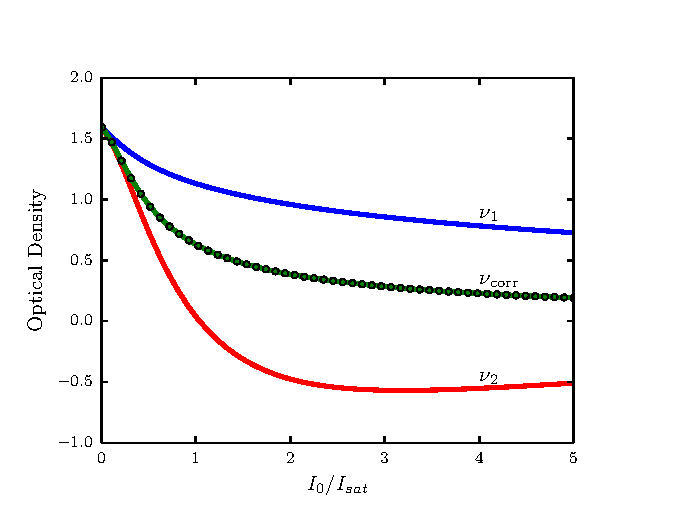
\includegraphics{figure7.pdf}
\caption{Predictions for optical depth as a function of probe intensity for an imaging time $t=100$\us. Note that the two versions of simulated optical depth, $OD_{corr1}$ (green line) and $OD_{corr2}$ (green dots) are virtually indistinguishable. }  
\label{fig:atomTravel}
\end{figure}

\subsection{Signal to noise optimization}
This simulation can be used to interpret experimentally obtained initial and final intensities. For a given imaging time, we create a look-up table of predicted optical depth as a function of probe intensity and atomic density. We can then find the observed optical depth on this table, with the given probe intensity, and infer the atomic density. The uncertainty in the measured intensities can be propagated through this procedure, and we can establish optimal imaging parameters to maximize the signal to noise ratio of this detection scheme. 
\par Here, the only source of measurement uncertainty we consider is the photon shot noise, which is Poisson distributed and has a standard deviation proportional to $\sqrt{N_p}$, where $N_p$ is the photon number. We then propagate this uncertainty through our correction scheme to get the uncertainty in our deduced value of $\sigma_0 n$. We define the signal to noise ratio (SNR) as $\sigma_0 n/\delta_{\sigma_0 n}$, where $ \delta_{\sigma_0 n}$ is the propagated measurement uncertainty.
\par As seen in Fig. \ref{fig:SNR}, after about 40\us{} extending the imaging time no longer yields appreciable improvement in signal to noise ratio. The advantage of imaging for 40\us{} as opposed to 10\us{} where the uncorrected model is appropriate is about a factor of  1.5 increase in SNR. We performed the experiments described in the second section at 40\us{} imaging time.
\begin{figure}
	\subfigure[]{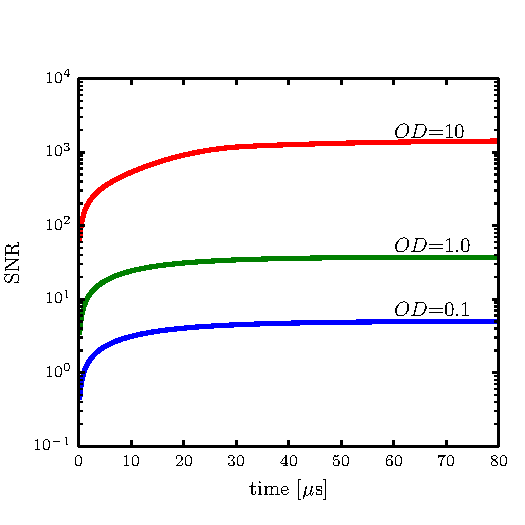
\includegraphics{figure9a.pdf}}
	\subfigure[]{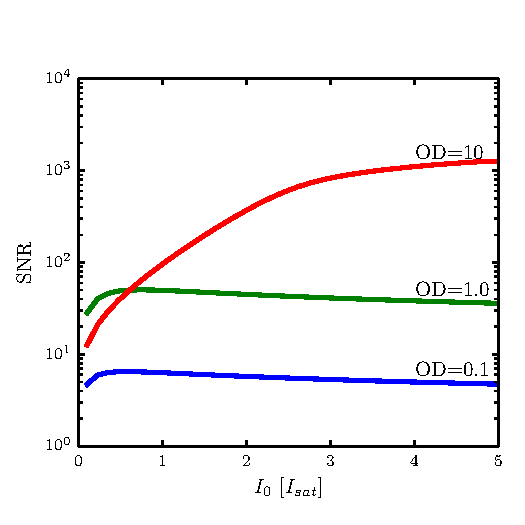
\includegraphics{figure9b.pdf}}
\caption{Signal to noise ratio (SNR) for three different optical depths after correcting for recoil induced detuning. a. SNR as a function of probe intensity $I_0/I_{sat}=5.0$ and b. SNR as a function of probe intensity for an imaging time of 50\us{}.}  
\label{fig:SNR}
\end{figure}

\subsection{Calibration of saturation intensity}
A key component of good detection is a well calibrated measurement apparatus. In this case, the measurement apparatus is a CCD camera used to take the absorption images. We used Point Grey's Flea3 camera.  Each camera pixel  converts tho photons it is exposed to, with some efficiency, into photoelectrons, and then to a digital signal, and integer we will call the number of 'counts'. The number of photons that hit a pixel and the number of 'counts' it outputs are directly proportional. However, the proportionality constant depends on many factors, such as the quantum efficiency of the camera, the photoelectric conversion factor of the camera, and the polarization of the probe light. 
\par The most accurate way to determine this factor is through a direct experiment. In the limit where the system is adequately described by Eq. (\ref{eq6}), only the ratio of the initial and final intensities matters, and thus this proportionality constant is irrelevant. In all other regimes, however, the ratio of the initial and final intensities to the saturation intensity also comes into play, making the proportionality constant significant. One way to approach this calibration is to determine the value of the saturation intensity in 'counts' per unit time. 
\par In order to calibrate the saturation intensity in camera counts per unit time, we take absorption images of a cloud of $^{40}K$ atoms at three different imaging times, 40us, 100us, and 200us, at varying probe intensities. We pick a small square in the center of the cloud, where the atomic density is approximately uniform, and average the initial and final intensities of each pixel in the square. Thus, for each image we obtain one $I_0$ and one $I_f$, in counts per microsecond. We then do a least squares fit of $OD_{corr}$, our simulated optical depth, to the data. The two fit parameters are the atomic density $n$ at the center of the cloud and the value of $I_{sat}$ in counts per microsecond. As seen in Fig. \ref{fig:isatCalib}, the model produces a good fit to the experimental data, and we obtain a calibration of the saturation intensity for our experiment. 
\begin{figure}
	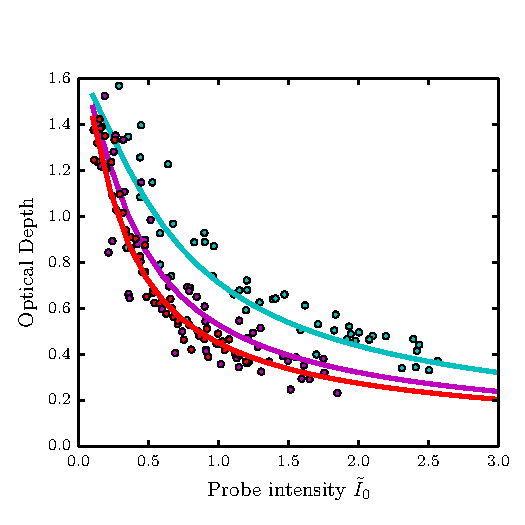
\includegraphics{figure8.pdf}
\caption{The optical depth as a function of probe intensity for three imaging times: $t=40$\us{} (blue),  $t=75$\us{} (green),  $t=100$\us{} (red). The dots represent experimental data and the lines represent the best fit of simulated data. The optimal fit parameters pictured are a $\sigma_0 n$ of 1.62 and saturation intensity of 29 counts/\us{}. }  
\label{fig:isatCalib}
\end{figure}


\section{S-wave scattering experiment}
In this section we describe our Fermi scattering experiment. We scattered two counter-propagating clouds of $^{40}K$ atoms and observed the resulting \swave halo of scattered atoms.  We measured the dependence of the scattered atomic fraction on the bias magnetic field in the vicinity of the Feshbach resonance. We used this data to extract the location of the magnetic fields resonance of 20.247(2) mT and a width of 1.0(1) mT.
\subsection{Experimental procedure}
Our cold Fermi cloud preparation was as follows. We prepared clouds of cold \K{} atoms in a hybrid \K{} and \Rb{} apparatus. We used a Zeeman slower to slow both species before being captured in a Magneto-Optical Trap (MOT). We allowed both species to cool in optical molasses for 2 miliseconds. Then, the \K{} atoms were optically pumped into the magnetically trappable $\ket{F=9/2, m_F=9/2}$ state. Both species were then loaded into a quadrupole magnetic trap, and cooled evaporatively. Since the \K{} atoms only interact very weakly with each other, they only re-thermalize due to interaction with \Rb{} atoms, and therefore the \Rb{} atoms are necessary to evaporatively cool \K{}. We then load the atoms into a crossed optical dipole trap, with trap frequencies of 39, 42, 124 Hz in the three spatial directions [I GOT THOSE FROM ROSS'S PAPER COULD BE WRONG FOR US]. We continued evaporative cooling by slowly ramping down the dipole trap. We then used adiabatic rapid passage (ARP) to transfer the \Rb{} atoms from the $\ket{F=2, m_F=2}$ state to the  $\ket{F=1, m_F=-1}$ absolute ground state. This state was chosen to minimize spin changing collisions with \K{} atoms during any further evaporation.  We then briefly shined an on-resonant probe light to force any remaining $F=2$ atoms out of the trap. We again used ARP to transfer the \K{} atoms into an equal superposition of $\ket{F=9/2,m_F=-9/2}$ and $\ket{F=9/2,m_F=-7/2}$, and further evaporated in the dipole trap. The $\ket{9/2,-9/2}$ and $\ket{9/2,-7/2}$ hyperfine states of \K{} were then used to study their Feshbach resonance. 

\par We then ramped the bias field in a two-step fashion to the desired value $B$ near the Feshbach resonance. To approach the field, we used a large pair of  coils in Helmholtz configuration to bring the magnetic field 0.59 mT of $B$. We held the atoms there to allow the eddy currents in the large coils to settle, and then used a smaller set of Helmholtz coils to hop the field the remaining 0.59 mT. We took two sets of data: one coming from below the resonance, where we hopped the large coils to $B-0.59 mT$ and used the small coils to hop up to the desired field, and one coming from above the resonance, where we hopped the large coils to  $B+0.59 mT$ and then used the small coils to hop the field down to the desired value. This allowed us to correct for losses due to molecule formation and three-body recombination \cite{Chin10}.
\par Once we had the Fermi cloud at the intended bias field, we imparted momentum in the $x$ direction to half of the cloud and in the $-x$ direction to the other half and observed them scatter as they moved through each other and separated. To impart the momentum, we used a double pulse sequence \cite{Wu05} of a near resonant 1-d retro-reflected optical lattice. The pulse sequence was optimized to transfer most of the atoms into the first two excited states of the lattice, giving them $\pm 2k_r$ of momentum, where $k_r$ is the recoil momentum of the lattice. Since the initial Fermi gas had a wide momentum spread (in contrast to a BEC, which has a very narrow momentum spread), and the lattice pulsing is a momentum dependent process, not all the atoms were successfully transferred into the 1st excited band of the lattice. We optimized our pulse times to minimize the number of atoms that remain in the zero momentum band of the lattice, but were not able to eliminate them completely. The optimized pulse times are 23\us{} for the first square pulse, 13\us{} off interval, and 12\us{} for the second square pulse. 
\par We then released the atoms from the trap and allowed 1ms for the two opposite momentum states within the cloud to pass through each other, scattering on the way. For the data taken coming from below the Feshbach resonance, we then simply ramped down the field and imaged the atoms. For the data taken coming from above the Feshbach resonance, we ramped the field back up through the resonance to recover any molecules that were created when the field was ramped from the attractive to the repulsive side of the resonance, and then quickly ramped the field back down and imaged the atoms. We use an imaging pulse of 40\us{}. 
\par The total time from the moment the atoms were released from the trap to when they were imaged, known as the time of flight, was 6.784 ms. In such an image, the location of each atoms is determined by how far it traveled in that time of flight, which is determined by its initial momentum when it was released from the trap. Therefore, this technique measures the momentum and not the position distribution of the atoms. 
\subsection{Methods}
\par We first corrected each image for recoil induced detuning using the simulation described above. We simulated a look-up table of predicted optical depths as a function of atomic column density and probe intensity. From our two absorption images we knew the probe intensity and optical depth for each pixel. We then used the simulated look-up table in an inverted fashion to deduce the atomic column density. An example of the effect of this correction procedure is shown in Fig. \ref{fig:SampleCorrection}.  To improve the signal and compensate for our shot to shot number fluctuations, we took 15 equivalent images for each data point and, after correcting, added them together.
\begin{figure}
	\subfigure[]{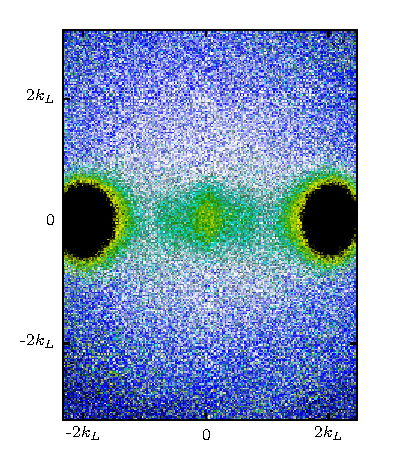
\includegraphics{figure10a.pdf}}
	\subfigure[]{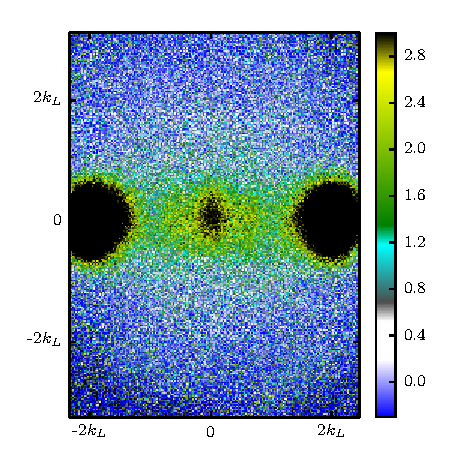
\includegraphics{figure10b.pdf}}
\caption{An example of our absorption image after 6.784ms time of flight. The 1-D lattice is along the horizontal direction at the center of our images. The two large clouds on the left and right are the atoms in the $\pm 2k_r$ momentum orders that passed through each other unscattered. The smaller cloud in the center is the atoms that remained in the lowest band of the lattice after pulsing, and thus obtained no momentum. The thin spread of atoms around these clouds is the atoms that underwent scattering.   This image was taken coming from below the Feshbach resonance at 20.07 mT. a. Raw optical density b. Optical density of the same image after correcting for recoil induced detuning}  
\label{fig:SampleCorrection}
\end{figure}
\par Once we acquired scattering images at a sufficient number of field values, we wanted to extract the fraction of atoms that underwent a single scattering event as a function of the bias field. We focused our attention on single-scattered atoms because, once an atom has scattered multiple times it is hard to determine precisely how many times it scattered, and therefore hard to deduce the scattering cross section.  An atom that underwent a single scattering event, however, is easily identified, as two atoms that scatter elastically will keep the same amplitude of momentum in an arbitrary direction. Therefore, an atom traveling at $2k_r$ to the right that collides with an atom traveling at $2k_r$ to the left will acquire a momentum of $2k_r$ in some direction, and in a time of flight image such atoms will lie in a spherical fashion around the center of mass -  the scattering halo, pictured in Fig. \ref{fig:halo}a. 
\begin{figure}
	\subfigure[]{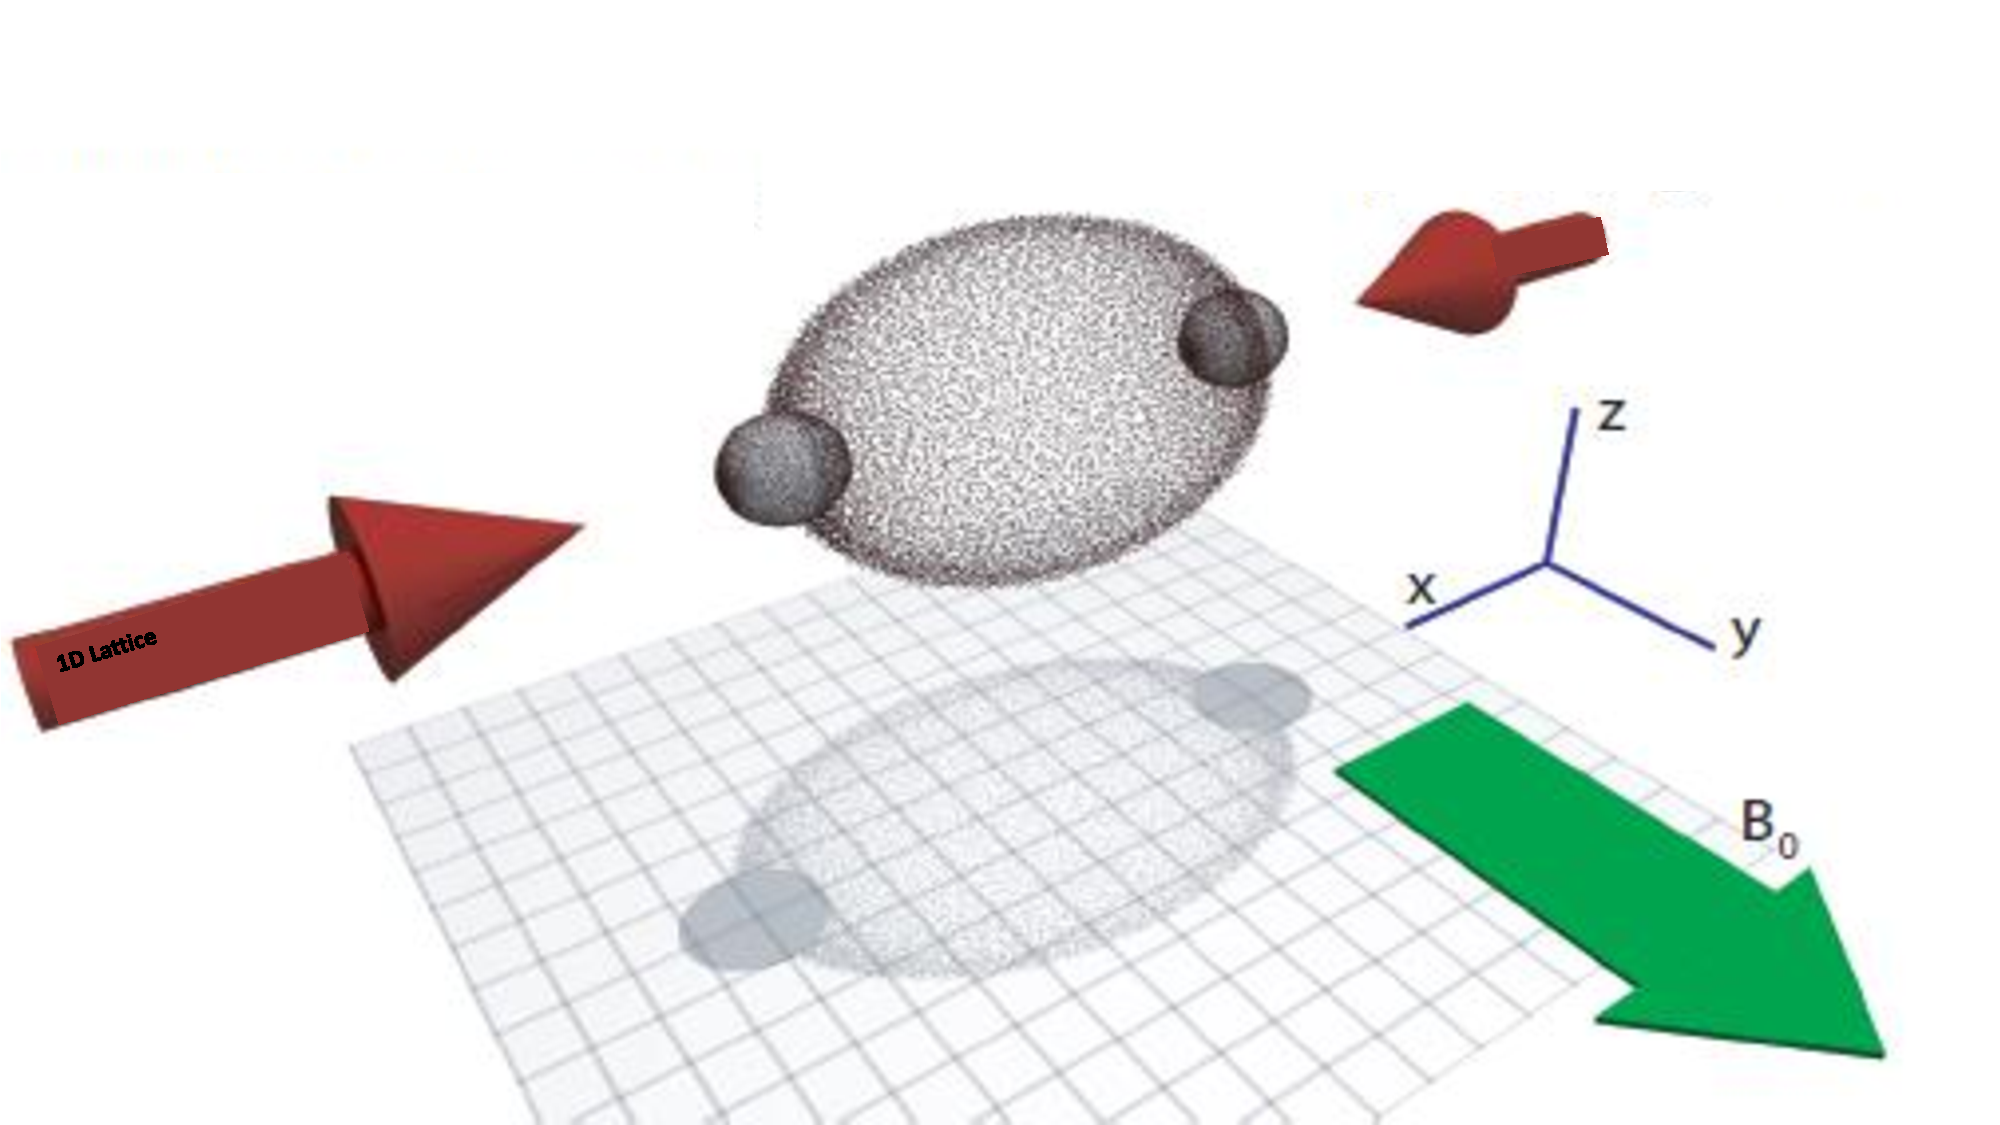
\includegraphics[scale=0.25]{Picture12.pdf}}
	\subfigure[]{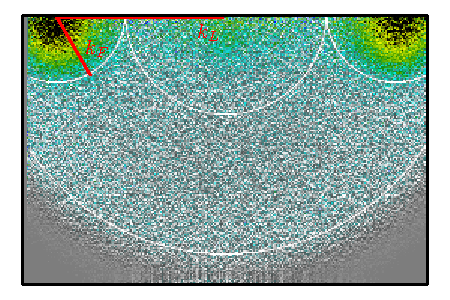
\includegraphics{figure12b.pdf}}
\caption{a. Our experimental setup. After time of flight, the two clouds traveling in opposite $x$ directions have separated and the atoms that underwent a single scattering event were evenly distributed in a scattering halo around the unscattered clouds. An absorption image captured the shadow the clouds cast onto a 2-d plane. b. Inverse Abel transformed image. The atoms within the Fermi radius $k_F$ of each unscattered cloud center are in the unscattered region and counted towards the total unscattered number. The atoms outside the radius $k_r-k_F$ but inside $k_r+k_F$ but outside the unscattered region are counted towards the number of single scattered atoms.   }  
\label{fig:halo}
\end{figure}
\par Absorption images captured the integrated column density along $z$, a projected 2-d atomic distribution. In order to extract the radial dependence of the 3-d distribution from the 2-d image, we performed a standard inverse Abel transform. The inverse Abel transform assumes a cylindrical symmetry, which was present in our case, with the axis of symmetry along $x$, defined by the lattice. We thus obtained the atomic distribution as a function of $r$, the radial distance from the scattering center, and $\theta$, the angle between $r$ and symmetry axis $x$, integrated over $\phi$, the azimuthal angle around the $x$ axis. 
\par We then extracted the number of atoms that went through a single scattering event $N_{scat}$, as a fraction of the total atom number $N_{tot}$, for each bias magnetic field value from the transformed images, as shown in Fig. \ref{fig:halo}b. We obtained the unscattered atom number by counting the number of atoms in the two unscattered clouds. We obtained the number of atoms that underwent a single scattering event by counting the number of atoms outside the Fermi radius of the unscattered clouds, but inside the arc created by rotating the Fermi momentum $k_F$ radius around the original center of the cloud. The total atom number in the image was the sum of those two.
\par We then used our data to deduce the resonant field value $B_0$ and width of the resonance  $\Delta$, the parameters in Eq. (\ref{feshbachEq}). To do this, we fit our data to a model. Since we were in the low energy regime, the scattering cross-section was given by $\sigma=4\pi a^2$. 
\par One way to think about the scattering cross-section $\sigma$ is that the probability $P_{scat}$ that a single particle will get scattered when incident on a cloud of atoms with a surface density of $\frac{N}{A}$ is given by $P_{scat}=\sigma \frac{N}{A}$. If this experiment is repeated 1000 times, the number of times the atom will get scattered is expected to be $N_{scat}=1000 \sigma \frac{N}{A}$.  In our case, half the initial cloud, with atoms number $N_{tot}/2$, is incident on the other half of the initial cloud, again with $N_{tot}/2$ atoms. Thus, the number of scattered atoms should be given by $N_{scat}=\frac{N_{tot}}{2} \sigma \frac{N_{tot}}{2}=\sigma \frac{N_{tot}^2}{4A}$, where $A$ is the cross-sectional area of the cloud. Assuming $A$ is constant for all our data, we can absorb the factor of 4A into our definition of $a_{bg}$, along with the $4\pi$, to obtain
\begin{equation}
\frac{N_{scat}}{N_{tot}^2}=\tilde{a}_{bg}^2\left(1-\frac{\Delta}{B-B_0}\right)^2 + C.
\label{eq:fit}
\end{equation}
\par We found that our imaging noise skewed towards the positive, giving rise to a small background offset. We accounted for this in our fit by including a constant offset parameter $C$. 
\subsection{Results}
Our final data is presented in Fig. \ref{fig:fittedFractions}. The red line is a best fit of the model given in Eq. (\ref{eq:fit}). The fit parameters we extracted are $\tilde{a}_{bg}=1.48e-3$, $\Delta = 1.0(1)$ mT, $B_0 = 20.247(2)$ mT, and $C=9.00e-5$. The error bars on the fitted data were obtained solely from photon shot noise of both absorption images propagated through our analysis.
The accepted values for the $^{40}K$ s-wave Feshbach resonance for the  $\ket{9/2,-9/2}$ and $\ket{9/2,-7/2}$ states are $B_0=20.210(7)$ mT and $\Delta=0.78(6)$ mT. The difference in our measurement may be a result of scattering with the center cloud that recieved no momentum kick, a process that was not taken into account by our analysis. 
\begin{figure}
	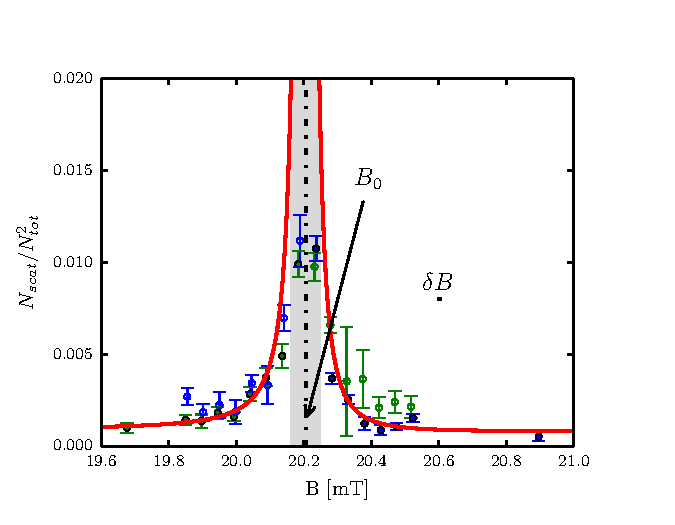
\includegraphics{figure11.pdf}
\caption{Normalized scattered population plotted versus bias field B. Green dots represent data taken coming from below the resonance, and blue dots represent the data taken coming from above the resonance. Red is the line of best fit, where data coming from above the resonance was used above the resonance and data coming from below the resonance was used below the resonance to create the fit. The regime where the scattering length is likely large enough for the atoms to behave hydrodynamically is shaded in gray. Data points in that region were not used in the fit, as there the assumption $\sigma\rho\ll1$, where $\rho$ is the atom number per unit area, is no longer valid. Values for the resonant field $B_0$ from literature and as found in this work are indicated.    }  
\label{fig:fittedFractions}
\end{figure}
\section{Conclusion}
We studied the effects of recoil-induced detuning effects on absorption images and found an optimal imaging time of ~40\us{} for $^{40}K$ atoms for noise minimization after corrections. We use these results to observe s-wave scattering halos of the Fermi gas around the Feshbach resonance and directly verify the resonance location and width. Our analysis can be used in any absorption imaging applications where signal to noise minimization is critical. We performed a new kind of measurement of the resonant magnetic field and with of a Feshbach resonance. 
\section*{Acknowledgments}
We thank Marcell Gall for helpful discussions. This work was partially supported by the ARO’s Atomtronics MURI, by the
AFOSR’s Quantum Matter MURI, NIST, and the NSF through the PFC at the JQI. B.K.S. is
a NIST-NRC Postdoctoral Research Associate. L.M.A. was supported by the NSF GRFP.

\section*{References}
\bibliography{refs}{}
\bibliographystyle{plain}

\end{document}

